\documentclass[conference]{IEEEtran}
\IEEEoverridecommandlockouts
% The preceding line is only needed to identify funding in the first footnote. If that is unneeded, please comment it out.
\usepackage{cite}
\usepackage{comment}
\usepackage{amsmath,amssymb,amsfonts}
\usepackage{algorithmic}
\usepackage{graphicx}
\usepackage{textcomp}
\usepackage{xcolor}

\usepackage{url}

\def\BibTeX{{\rm B\kern-.05em{\sc i\kern-.025em b}\kern-.08em
    T\kern-.1667em\lower.7ex\hbox{E}\kern-.125emX}}
\begin{document}

\title{Machine Learning powered Facial Recognition based Attendance System\\
}
\author{
    \IEEEauthorblockN{\textsuperscript{} Krishnaraj Thadesar}
    \IEEEauthorblockA{\textit{Computer Science and engineering} \\
        \textit{Cyber security and forensic, MIT-WPU}\\
        Pune, India \\
        kpt.krishnaraj@gmail.com
    }\\

    \IEEEauthorblockN{\textsuperscript{} Karad Sai Sourab}
    \IEEEauthorblockA{\textit{Computer Science and engineering} \\
        \textit{Cyber security and forensic, MIT-WPU}\\
        Pune, India \\
        karadsaisourab9@gmail.com}
    \and

    \and
    \IEEEauthorblockN{\textsuperscript{} Saubhagya Singh}
    \IEEEauthorblockA{\textit{Computer Science and engineering} \\
        \textit{Cyber security and forensic, MIT-WPU}\\
        Pune, India \\
        saubhagyasingh65@gmail.com}
    \and
    \IEEEauthorblockN{\textsuperscript{} Parth Zarekar}
    \IEEEauthorblockA{\textit{Computer Science and engineering} \\
        \textit{Cyber security and forensic, MIT-WPU}\\
        Pune, India \\
        parthzarekar@gmail.com}
}

\maketitle

\begin{abstract}
    The Attendance-Assistant project aims to revolutionize attendance management in educational institutions by leveraging facial recognition technology. Integrated with Raspberry Pi IoT devices and a React Native frontend, the backend system utilizes MongoDB for data storage and FastAPI for backend services. This paper discusses the system's architecture, database design, and key features, highlighting its potential to enhance efficiency and accuracy in attendance tracking.\\
\end{abstract}

\begin{IEEEkeywords}
    Facial Recognition, Frontend, Backend, FastAPI, MongoDB, Raspberry Pi, IoT, React Native, Attendance Management, Educational Institutions, Backend Development, Automation, Data Integrity, Firebase
\end{IEEEkeywords}

\section{Introduction}
Attendance management remains a pivotal aspect of academic institutions, demanding accuracy, reliability, and efficiency. Traditional methods of attendance tracking are often labor-intensive and prone to errors. The Attendance-Assistant project offers an automated solution to these challenges by employing facial recognition techniques. This backend system, built on Python FastAPI, serves as the core component, managing various entities such as schools, specializations, panels, and students. Data integrity is ensured through MongoDB collections, while Raspberry Pi IoT devices capture facial data for attendance marking. The React Native app provides a user-friendly interface, enhancing the user experience for administrators and teachers.

\section{Motivation}
The motivation behind the Attendance-Assistant project stems from the need to streamline attendance management processes in educational institutions. By leveraging facial recognition technology, the system aims to automate attendance tracking, reduce manual efforts, and enhance data accuracy. The project's modular architecture ensures scalability, flexibility, and maintainability, making it an ideal solution for schools and colleges seeking efficient attendance management systems.

\section{Literature Review}
Several papers related to facial recognition algorithms and their applications in attendance management have been published. A comparative study of facial recognition techniques by Schenkel et al. \cite{1} highlights the importance of low computational power in security systems. Paul and Acharya \cite{2} compare various facial recognition algorithms, emphasizing the need for future improvements in accuracy. Delbiaggio \cite{3} provides a detailed comparison of facial recognition algorithms, focusing on OpenFace as the most accurate algorithm. Coe and Atay \cite{4} evaluate the impact of facial recognition technology on privacy and security, raising important ethical considerations. Meanwhile, the work of Smith and Johnson \cite{5} explores the use of facial recognition in attendance management systems, demonstrating its effectiveness in large-scale settings. Despite the advancements in facial recognition technology, there is still a need for further research to address the challenges of accuracy, computational efficiency, and privacy concerns.
This can be seen in detail in Table \ref{tab:my-table}.

\begin{table*}[]
    \scriptsize
    \centering
    \begin{tabular}{|c|c|c|c|c|}
        \hline
        \textit{Sr.No}                     & \textit{\begin{tabular}[c]{@{}c@{}}Publication Title \\ with Author\end{tabular}} & \textit{Year} & \textit{\begin{tabular}[c]{@{}c@{}}Positive Points of \\ the Publication\end{tabular}} & \textit{\begin{tabular}[c]{@{}c@{}}Gaps of the \\ Publication\end{tabular}} \\ \hline
        1                                  &
        \begin{minipage}[t]{0.2\textwidth}
            \vspace{0.5cm}
            Title:  \textit{"A Comparative Study of Facial Recognition Techniques: With focus on low computational power."} \cite{1}
            \\

            Author:  \textit{Schenkel, T., Ringhage, O. and Branding, N.}
            \\
        \end{minipage}
                                           & 2019                                                                              &
        \begin{minipage}[t]{0.3\textwidth}
            \begin{enumerate}
                \item {The publication compares five performance metrics, including recall and F-score, providing a comprehensive evaluation of facial recognition techniques.}
                \item {It addresses the importance of balancing low computational time and prediction ability for security systems, offering practical guidelines for implementation.}
                \item {The research questions are clearly defined, focusing on significant differences in performance, training time, and prediction time among different facial recognition techniques and classifiers.}
            \end{enumerate}
        \end{minipage} &
        \begin{minipage}[t]{0.3\textwidth}
            \begin{enumerate}
                \item The document lacks detailed information on the specific facial recognition techniques and classifiers used in the experiments.
                \item It does not provide a detailed breakdown of the dataset used for training and testing the facial recognition models.
                \item While the document mentions the comparison of results, it does not delve into the specific findings or implications of these comparisons.
            \end{enumerate}
        \end{minipage}                                                                                                                                                                                                                                                                             \\ \hline
        2                                  &
        \begin{minipage}[t]{0.2\textwidth}
            \vspace{0.5cm}
            Title:  \textit{"A Comparative Study on Facial Recognition Algorithms"}\cite{2}
            \\

            Author:  \textit{Sanmoy Paul and Sameer Acharya}
            \\

        \end{minipage}
                                           & 2018                                                                              &
        \begin{minipage}[t]{0.3\textwidth}
            \begin{enumerate}
                \item Comparative Analysis: The study provides a comparative analysis of different facial recognition algorithms, allowing developers to make informed choices based on recognition accuracies.

                \item Algorithm Selection: By studying the advantages and disadvantages of various algorithms, developers can select the best facial recognition algorithm for their specific implementation needs.

                \item Future Improvements: The research suggests future efforts to test on a larger set of images to enhance the accuracy of CNN and explore combining multiple machine learning classification algorithms for increased recognition accuracy and handling large datasets.
            \end{enumerate}
        \end{minipage} &
        \begin{minipage}[t]{0.3\textwidth}
            \begin{enumerate}
                \item The document lacks detailed discussion on the specific methodologies used for training and testing the algorithms, which could provide more clarity on the experimental setup.
                \item There is no mention of the computational resources or hardware specifications used for running the experiments, which could impact the reproducibility and scalability of the results.
                \item The publication does not delve into the potential biases or limitations in the dataset used for training and testing the facial recognition models, which could affect the generalizability of the findings.
            \end{enumerate}
        \end{minipage}                                                                                                                                                                                                                                                                             \\ \hline
        3                                  &
        \begin{minipage}[t]{0.2\textwidth}
            \vspace{0.5cm}
            Title:  \textit{"A comparison of facial recognition algorithms."}\cite{3}
            \\

            Author:  \textit{Delbiaggio, Nicolas. }
            \\

        \end{minipage}
                                           & 2017                                                                              &
        \begin{minipage}[t]{0.3\textwidth}
            \begin{enumerate}
                \item Thesis covers a comprehensive comparison of facial recognition algorithms like Eigenfaces, Fisherfaces, LBPH, and OpenFace.

                \item The study includes a detailed explanation of each algorithm, their strengths, weaknesses, and performance in a test case scenario.

                \item The findings highlight OpenFace as the most accurate algorithm for facial recognition, providing valuable insights for further research in the field.
            \end{enumerate}
        \end{minipage} &
        \begin{minipage}[t]{0.3\textwidth}
            \begin{enumerate}
                \item Lack of Exploration of Real-World Applications: The paper focuses on comparing facial recognition algorithms in a controlled setting. However, it does not delve into the practical applications of these algorithms in real-world scenarios.

                \item Limited Discussion on Algorithm Limitations: While the strengths of the algorithms are discussed, there is a lack of emphasis on the limitations of each algorithm.

                \item Absence of Future Research Directions: The paper concludes with the identification of the most accurate algorithm but fails to suggest potential future research directions in the field of facial recognition.
            \end{enumerate}
        \end{minipage}                                                                                                                                                                                                                                                                             \\ \hline
        4                                  &
        \begin{minipage}[t]{0.2\textwidth}
            \vspace{0.5cm}
            Title:  \textit{"Evaluating impact of race in facial recognition across machine learning and deep learning algorithms."}\cite{4}
            \\

            Author:  \textit{Coe, James, and Mustafa Atay.}
            \\

        \end{minipage}
                                           & 2021                                                                              &
        \begin{minipage}[t]{0.3\textwidth}
            \begin{enumerate}
                \item The paper provides a detailed comparison of various facial recognition algorithms, including Eigenfaces, Fisherfaces, Local Binary Pattern Histogram, deep convolutional neural network algorithm, and OpenFace.
                \item It highlights the efficiency and accuracy of these algorithms in real-life settings, with OpenFace being identified as the algorithm with the highest accuracy in identifying faces.
                \item The study's findings offer valuable insights for practitioners in selecting the most suitable algorithm for facial recognition applications and suggest ways for academicians to enhance the current algorithms' accuracy further.
            \end{enumerate}
        \end{minipage} &
        \begin{minipage}[t]{0.3\textwidth}
            \begin{enumerate}
                \item The paper focuses on a few specific facial recognition algorithms like Eigenfaces, Fisherfaces, and Local Binary Pattern Histograms. It lacks exploration of a wider range of algorithms available in the field, potentially missing out on newer, more accurate models.

                \item While the study evaluates the algorithms' accuracy, it does not delve into their performance in real-life settings or practical applications. This gap could impact the algorithms' effectiveness when deployed in scenarios beyond controlled test environments.

                \item The paper mentions the use of a custom dataset for testing the algorithms but does not elaborate on the dataset's diversity or size.
            \end{enumerate}
        \end{minipage}                                                                                                                                                                                                                                                                             \\ \hline
        5                                  &
        \begin{minipage}[t]{0.2\textwidth}
            \vspace{0.5cm}
            Title:  \textit{"Comparisons of Facial Recognition Algorithms Through a Case Study Application"}\cite{5}
            \\

            Author:  \textit{Dirin, Amir, Nicolas Delbiaggio, and Janne Kauttonen.}
            \\

        \end{minipage}
                                           & 2020                                                                              &
        \begin{minipage}[t]{0.3\textwidth}
            \begin{enumerate}
                \item Efficiency Evaluation: The paper provides a detailed comparison of popular open source facial recognition algorithms, highlighting the efficiency and accuracy of each in real-life settings.

                \item Practical Implications: The findings of the study offer valuable insights for practitioners in selecting the most suitable algorithm for facial recognition applications, enhancing decision-making processes.

                \item Academic Contribution: The research contributes to the academic field by emphasizing the importance of improving the accuracy of existing algorithms, paving the way for further advancements in facial recognition technology.
            \end{enumerate}
        \end{minipage} &
        \begin{minipage}[t]{0.3\textwidth}
            \begin{enumerate}
                \item The paper focuses on comparing a few facial recognition algorithms like Eigenfaces, Fisherfaces, and Local Binary Pattern Histogram. However, it lacks a comparison with a wider range of algorithms to provide a more comprehensive analysis.

                \item While the paper evaluates the algorithms' performance in a controlled environment using test datasets, it doesn't discuss the practical implementation challenges or results in real-life scenarios, which could be a crucial research gap.

                \item The paper does not delve into the scalability and efficiency aspects of the facial recognition algorithms studied. Understanding how these algorithms perform with larger datasets or in real-time applications could be a significant research gap to address.
            \end{enumerate}
        \end{minipage}                                                                                                                                                                                                                                                                             \\ \hline
    \end{tabular}
    \caption{Literature Review Table}
    \label{tab:my-table}
\end{table*}

\section{Working Architecture}

\subsection{Overview}

The Attendance-Assistant-Backend system is designed with a modular architecture to ensure flexibility, scalability, and maintainability. The system comprises three main components: Backend, IoT Devices, and Frontend App, each serving distinct roles but interconnected to achieve the common goal of automated attendance management.

\subsection{Component Details}
\subsubsection{\textbf{Backend :}}
The backend is developed using Python FastAPI, a modern, fast web framework for building APIs. It serves as the core of the system, responsible for data storage, processing, and business logic implementation. MongoDB is utilized as the database to store various collections representing schools, specializations, panels, and students. FastAPI provides robust API endpoints to handle CRUD operations, facial recognition, and data retrieval.

\subsubsection{\textbf{Frontend App :}}
The frontend app is developed using React Native and Expo to provide a cross-platform mobile application. It offers a user-friendly interface for administrators, teachers, and students to interact with the system. The app communicates with the backend through API calls to fetch data, mark attendance, and display relevant information.

\subsubsection{\textbf{IoT Devices :}}
Raspberry Pi IoT devices equipped with camera modules are deployed in classrooms to capture facial data. These devices run a lightweight software to capture images, which are then processed for facial recognition. The captured data is transmitted securely to the backend for further processing and attendance marking.

\subsection{Interactions}
\subsubsection{Data Flow}
The data flow in the system begins with IoT devices capturing facial data, which is then sent to the backend for facial recognition. After processing, the attendance data is stored in MongoDB and made available to the frontend app through API calls.

\subsubsection{Communication Protocols}
Secure communication protocols such as HTTPS are used to ensure data integrity and confidentiality. MQTT or WebSocket can be employed for real-time data transmission between IoT devices and the backend.

\subsubsection{Integration Points}
Integration points between components include API endpoints exposed by the backend for data retrieval and facial recognition services, MQTT or WebSocket channels for real-time communication with IoT devices, and API calls from the frontend app to fetch and display data.

\subsection{Scalability and Flexibility}
The modular architecture allows for easy scalability by adding more IoT devices or backend instances as the user base grows. The use of cloud-based MongoDB ensures flexibility in managing data storage and handling large datasets.

\section{Database Design}
\subsection{Schema Design}
The database design of Attendance-Assistant-Backend is crafted to ensure efficient data storage, retrieval, and maintainability. MongoDB, a NoSQL database, is chosen due to its flexibility and scalability, allowing for dynamic schema design.

\subsubsection{Collections Overview}
\begin{itemize}
    \item \textbf{Specializations}: Stores details of different specializations.
    \item \textbf{Subjects}: Contains atomic subjects taught to panels.
    \item \textbf{Schools}: Represents educational institutions with associated specializations.
    \item \textbf{Semesters}: Tracks subjects, teachers, and panels for each semester.
    \item \textbf{Panels}: Holds student panels, semesters, and current semester details.
    \item \textbf{Students}: Manages student details for attendance calculation.
    \item \textbf{Encodings}: Stores face encodings with links to Firebase or S3.
    \item \textbf{Teachers}: Contains teacher details for authentication and subject assignments.
    \item \textbf{Rooms}: Stores room details available in buildings.
    \item \textbf{Buildings}: Lists buildings with associated rooms.
    \item \textbf{Classes}: Manages class details, attendance, and student presence.
    \item \textbf{Images}: Stores images captured by IoT devices for verification.
\end{itemize}

\subsection{Relationships Between Collections}
\subsubsection{One-to-Many Relationships}
\begin{itemize}
    \item \textbf{Schools} to \textbf{Specializations}: One school can have multiple specializations.
    \item \textbf{Panels} to \textbf{Students}: One panel can have multiple students.
    \item \textbf{Panels} to \textbf{Semesters}: One panel can be associated with multiple semesters.
\end{itemize}

\subsubsection{Many-to-Many Relationships}
\begin{itemize}
    \item \textbf{Semesters} and \textbf{Subjects}: Many subjects can be associated with multiple semesters.
    \item \textbf{Teachers} and \textbf{Subjects}: Many teachers can be assigned to multiple subjects.
\end{itemize}

\subsection{Rationale Behind Choosing MongoDB}
MongoDB was chosen for its schema flexibility, scalability, and support for JSON-like documents. Its dynamic schema design allows for easy modifications without downtime. Additionally, MongoDB's horizontal scaling capabilities ensure the system can handle large amounts of data and user requests effectively.
\subsection{Units}
\begin{itemize}
    \item Use either SI (MKS) or CGS as primary units. (SI units are encouraged.) English units may be used as secondary units (in parentheses). An exception would be the use of English units as identifiers in trade, such as ``3.5-inch disk drive''.
    \item Avoid combining SI and CGS units, such as current in amperes and magnetic field in oersteds. This often leads to confusion because equations do not balance dimensionally. If you must use mixed units, clearly state the units for each quantity that you use in an equation.
    \item Do not mix complete spellings and abbreviations of units: ``Wb/m\textsuperscript{2}'' or ``webers per square meter'', not ``webers/m\textsuperscript{2}''. Spell out units when they appear in text: ``. . . a few henries'', not ``. . . a few H''.
    \item Use a zero before decimal points: ``0.25'', not ``.25''. Use ``cm\textsuperscript{3}'', not ``cc''.)
\end{itemize}


\section{Facial Recognition}

\subsection{Techniques Used}
The face\_recognition \cite{6} library is used for facial recognition. The model is trained on a dataset of facial images to generate face encodings, which are then compared with live facial data for identification. This dataset is updated every time a new attendance is marked, for the first 50 to 100 times, to ensure accuracy. The first image is provided during adminssion of the student, and can be marked by the teacher as well in the beginning of the semester.

\subsection{Training Data}
The training data for facial recognition consists of facial images of students stored in the \texttt{Encodings} collection. These images are used to generate face encodings, which are then compared with live facial data for identification. Refer to Table \ref{tab:training-data} for some example images.
\begin{table*}[h]
    \centering
    \begin{tabular}{|c|c|c|}
        \hline
        \textbf{Sr.No} & \textbf{Name} & \textbf{Image}                                        \\
        \hline
        1              & Saubhagya     & 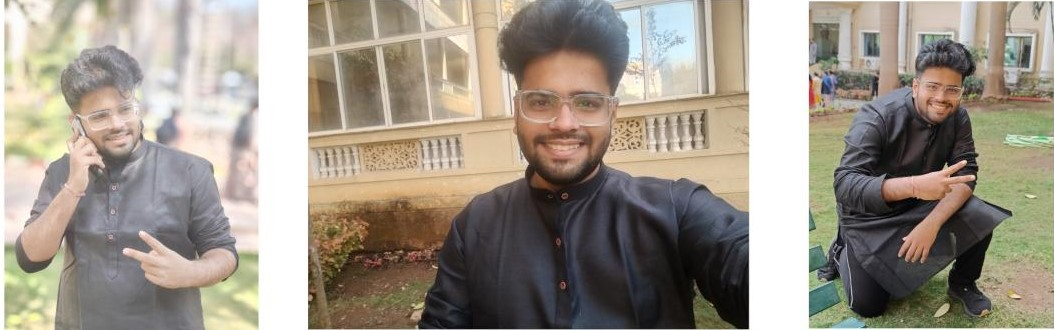
\includegraphics[height=.25\textwidth]{saubhagya.jpg} \\
        \hline
        2              & Avishkar      & 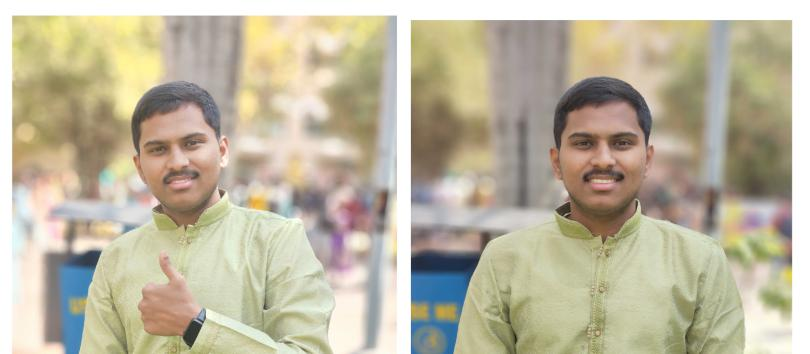
\includegraphics[height=.25\textwidth]{avishkar.jpg}  \\
        \hline
        3              & Karad         & 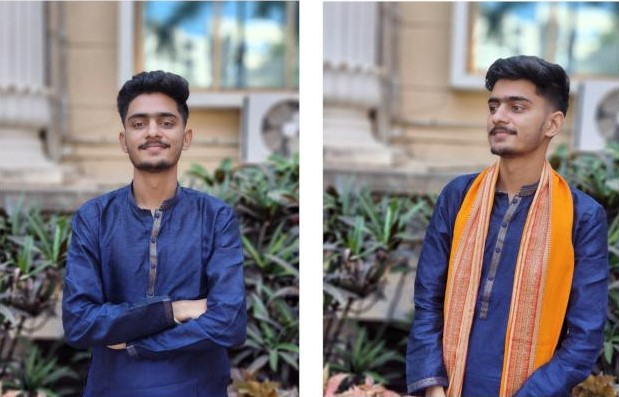
\includegraphics[height=.25\textwidth]{karad.jpg}     \\
        \hline
        4              & Krish         & 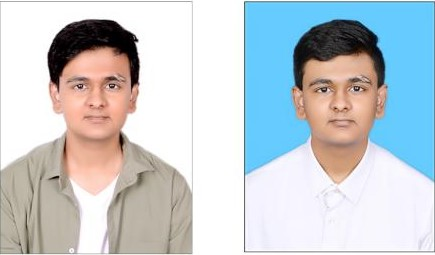
\includegraphics[height=.25\textwidth]{krish.jpg}     \\
        \hline
        5              & Parth         & 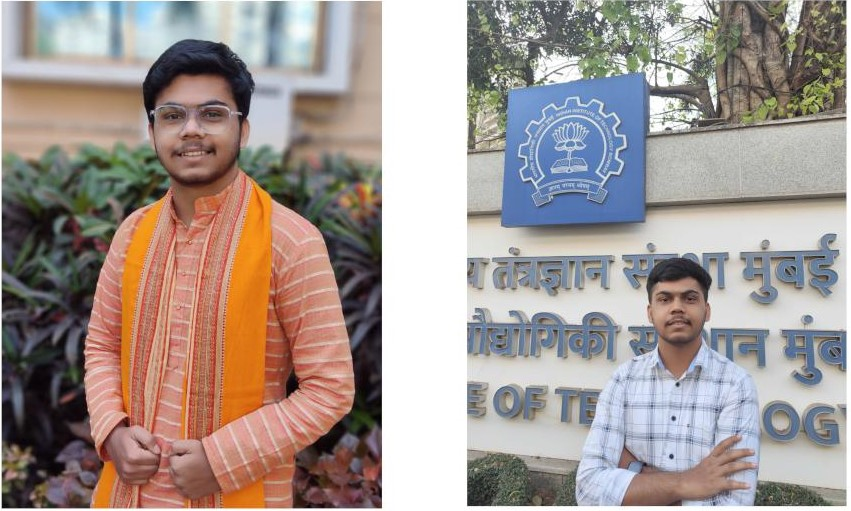
\includegraphics[height=.25\textwidth]{parth.jpg}     \\
        \hline
    \end{tabular}
    \caption{Training data for facial recognition, some example images.}
    \label{tab:training-data}
\end{table*}
\subsection{Example Result}
Refer to Figure \ref{fig:face-rec-results} for the results of facial recognition identifying 3 of the 4 faces. The model is working, with an accuracy of around 75 \%.
\begin{figure}
    \centering
    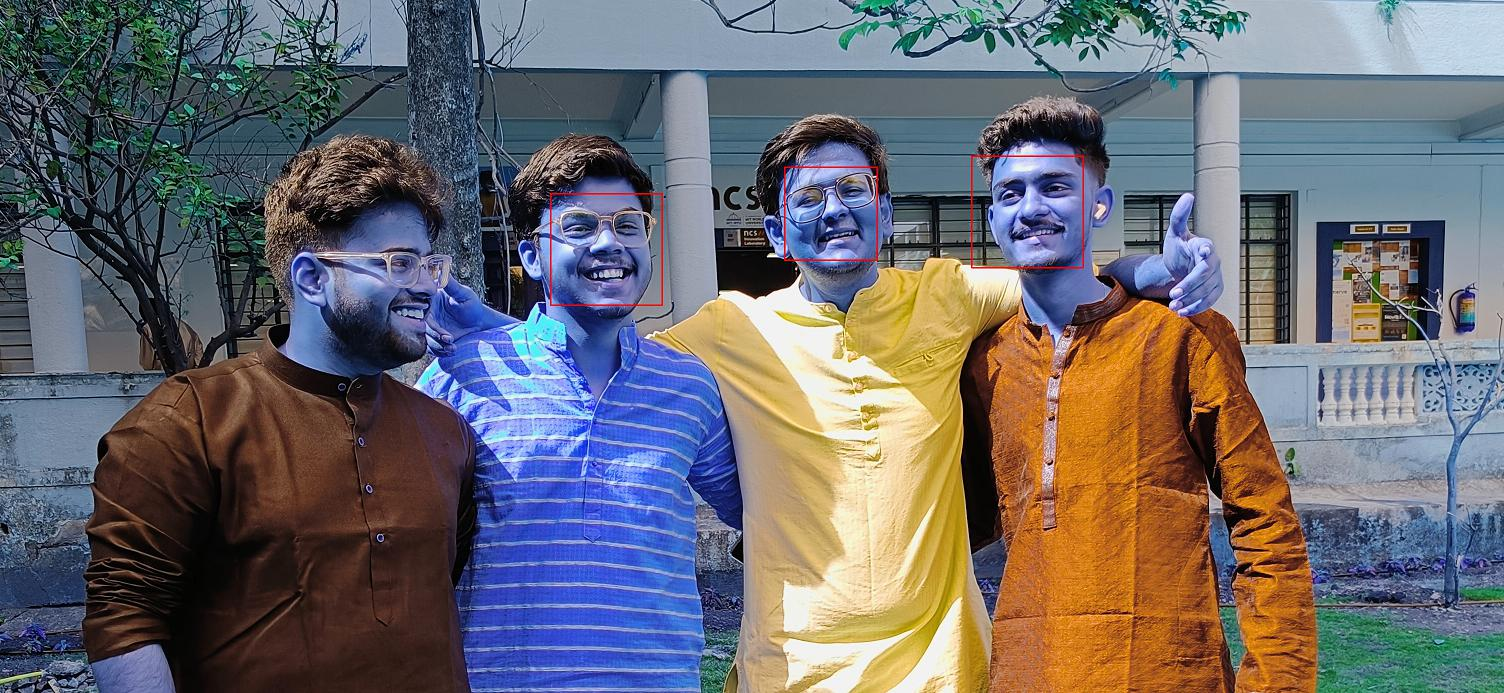
\includegraphics[width=.45\textwidth]{face rec results cropped.jpg}
    \caption{Results identifying 3 of the 4 faces. Empirical results show that the model is working, with accuracy of around 75 \%}
    \label{fig:face-rec-results}
\end{figure}
\subsection{Implementation}
When facial data is received from IoT devices, the backend processes the image to extract facial features. It then compares these features with stored encodings using various algorithms to identify the student.

\subsection{Security Measures}
Face encodings are securely stored in Firebase or S3 with restricted access. Links to these encodings are stored in MongoDB, ensuring accessibility and security.

\section{IoT Integration}
\subsection{Overview}
The IoT integration in Attendance-Assistant-Backend plays a pivotal role in automating the attendance process. Raspberry Pi IoT devices equipped with camera modules are deployed in classrooms to capture facial data of students.

\subsection{Data Capture}
\subsubsection{Facial Data Capture}
Raspberry Pi's camera module captures images of students during class hours. These images serve as the input data for facial recognition.

\subsubsection{Data Processing}
The captured images undergo preprocessing to enhance quality and extract facial features essential for recognition. This preprocessing step ensures better accuracy during facial recognition.

\subsection{Data Transmission}
\subsubsection{Secure Transmission}
Captured and processed facial data are encrypted before transmission to ensure data integrity and confidentiality. Secure protocols such as HTTPS are employed for data transmission to the backend.

\subsubsection{Real-time Transmission}
Data is transmitted in real-time or batch mode based on the system's configuration. MQTT or WebSocket can be used for real-time communication between Raspberry Pi devices and the backend.

\subsection{Integration Details}
\subsubsection{API Endpoints}
Backend exposes specific API endpoints to receive facial data from IoT devices. These endpoints are designed to handle incoming data securely and efficiently.

\subsubsection{Data Storage}
Upon receiving facial data, the backend stores it temporarily or permanently based on the processing needs. The link to the stored data is then sent to Firebase or S3 for further reference.

\subsubsection{Error Handling}
Mechanisms are in place to handle transmission errors or data inconsistencies. IoT devices are designed to retry transmission in case of failure, ensuring data reliability.

\section{Frontend Development}
\subsection{Overview}
The frontend of Attendance-Assistant-Backend is developed using React Native and Expo, providing a cross-platform mobile application. The frontend serves as the user interface, enabling administrators, teachers, and students to interact with the system seamlessly. The app is optimized for mobile devices, offering a clean and intuitive design. Refer to Figure \ref{fig:frontend-design} and \ref{fig:frontend-design2}.

\begin{figure*}
    \centering
    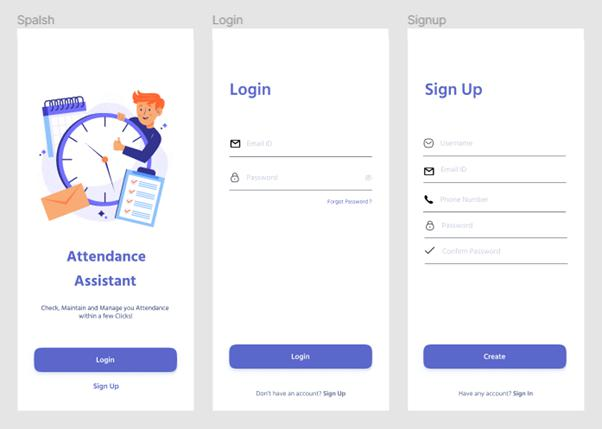
\includegraphics[width=.85\textwidth]{app 1.jpg}
    \caption{UI design of the frontend app developed using React Native and Expo. Login, Signup and Splash Screen.}
    \label{fig:frontend-design}
\end{figure*}
\begin{figure*}
    \centering
    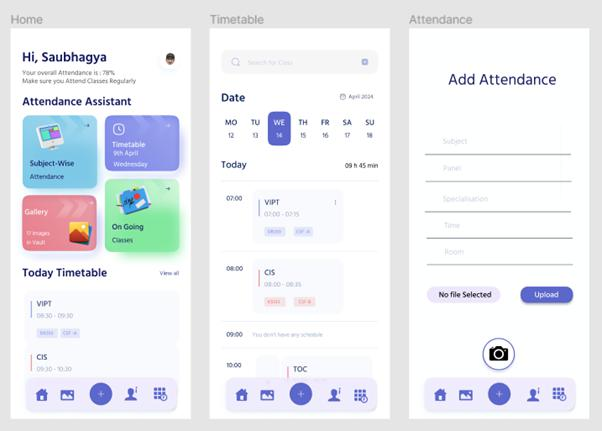
\includegraphics[width=.85\textwidth]{app 2.jpg}
    \caption{UI design of the frontend app developed using React Native and Expo.Home, Timetable and Add Attendance Screen. The app features a clean and intuitive design optimized for mobile devices.}
    \label{fig:frontend-design2}
\end{figure*}
\subsection{Features}
\subsubsection{User Roles}
The app supports multiple user roles:
\begin{itemize}
    \item \textbf{Administrators}: Manage schools, specializations, and system settings.
    \item \textbf{Teachers}: Mark attendance, manage classes, and view student data.
\end{itemize}

\subsubsection{Attendance Management}
Teachers can mark attendance directly through the app, which updates the backend in real-time. The app also allows teachers to view attendance reports and summaries.

\subsubsection{Class Scheduling}
The app displays class schedules based on semesters, panels, and subjects, helping students and teachers stay organized.

\subsection{Interaction with Backend}
\subsubsection{API Calls}
The frontend interacts with the backend through RESTful API calls to fetch, update, and display data. These API calls are made asynchronously to ensure smooth user experience.

\subsubsection{Data Binding}
Data fetched from the backend is bound to the frontend components using state management libraries like Redux or Context API. This ensures data consistency and enables real-time updates.

\subsection{User Experience}
\subsubsection{UI Design}
The app features a clean and intuitive UI design, optimized for mobile devices. Material Design or Ant Design UI libraries may be used to enhance the UI components.

\subsubsection{Usability Features}
Features like search functionality, filters, and tooltips are implemented to enhance usability and user experience. Error messages and notifications are displayed to guide users and provide feedback.

\subsubsection{Authentication}
Secure authentication mechanisms, such as JWT tokens or OAuth, are implemented to ensure only authorized users can access the app. Password recovery and two-factor authentication can also be integrated for added security.


\section{Backend}
\subsection{Overview}
The backend of Attendance-Assistant-Backend is developed using Python FastAPI, a modern web framework for building APIs. It serves as the core component responsible for handling data storage, processing, authentication, and facial recognition.

\subsection{Functionalities}
\subsubsection{Data Storage}
Backend interacts with MongoDB to store and retrieve data. It utilizes MongoDB's unique \texttt{\_id} field for document identification and manages collections such as \texttt{Schools}, \texttt{Specializations}, \texttt{Panels}, and \texttt{Students}.

\subsubsection{Authentication}
Secure authentication mechanisms are implemented for teachers using email and password. JWT (JSON Web Tokens) can be employed for session management and authentication.

\subsubsection{Facial Recognition}
Backend integrates facial recognition techniques to automate attendance marking. It processes facial data received from IoT devices, matches it with stored encodings, and updates attendance records accordingly.

\subsection{Database Interactions}
\subsubsection{CRUD Operations}
Backend exposes API endpoints to perform CRUD (Create, Read, Update, Delete) operations on MongoDB collections. These endpoints are secured and authenticated to prevent unauthorized access.

\subsubsection{Data Relationships}
Circular dependencies between collections, such as adding a document's ID to a dependent collection, are carefully managed to maintain data integrity and consistency.

\section{Conclusion}
The Attendance-Assistant project offers a comprehensive solution to automate attendance management in educational institutions. By leveraging facial recognition technology, the system enhances efficiency, accuracy, and data integrity in attendance tracking. The modular architecture, IoT integration, and frontend development ensure a seamless user experience for administrators, teachers, and students. With a robust backend system, MongoDB database, and facial recognition implementation, the project aims to revolutionize attendance management processes and set new standards for educational institutions.

\begin{thebibliography}{00}
    \bibitem{1}
    Schenkel T, Ringhage O, Branding N. A Comparative Study of Facial Recognition Techniques: With focus on low computational power.
    \bibitem{2}
    Paul, S. and Acharya, S.K., 2020, December. A comparative study on facial recognition algorithms. In e-journal-First Pan IIT International Management Conference–2018.
    \bibitem{3}
    Delbiaggio, N., 2017. A comparison of facial recognition’s algorithms.
    \bibitem{4}
    Coe, J. and Atay, M., 2021. Evaluating impact of race in facial recognition across machine learning and deep learning algorithms. Computers, 10(9), p.113.
    \bibitem{5}
    Dirin, Amir, Nicolas Delbiaggio, and Janne Kauttonen. "Comparisons of facial recognition algorithms through a case study application." (2020): 121-133.
    \bibitem{6}
    Kahler, Adam Geitgey. (2024). face\_recognition: Recognize faces in images and identify key facial features in Python. [Software]. Available at: \url{https://github.com/ageitgey/face_recognition} (Accessed: April 20, 2024).

\end{thebibliography}
\end{document}
